\documentclass[10pt]{article}
\usepackage{tikz}
\usetikzlibrary{arrows.meta, positioning}

\usepackage{parskip}
\usepackage[margin=1in]{geometry} 
\usepackage{amsmath,amsthm,amssymb, graphicx, multicol, array}
\usepackage{enumitem}
\usepackage{amssymb}
\usepackage{float}
\usepackage{href-ul}
 
\newcommand{\N}{\mathbb{N}}
\newcommand{\Z}{\mathbb{Z}}
 
\newenvironment{problem}[2][Problem]{\begin{trivlist}
\item[\hskip \labelsep {\bfseries #1}\hskip \labelsep {\bfseries #2.}]}{\end{trivlist}}

\begin{document}
 
\title{Vector Autoregression (VAR)}
\author{Jakob Sverre Alexandersen\\
GRA4159 Trends, Cycles \& Signals Extraction\\
Lecture 8}
\maketitle

\tableofcontents
\newpage

\section{Recap}
\begin{itemize}
    \item We know the difference between stationary and non-stationary variables and time series processes, such as AR, MA, RW 
    \item We also know why we sometimes want to focus on trend and cycle decompositions and how to cmopute them using different methods 
\end{itemize}
But, we only have been working with univariate models, i.e., just one outcome variable. Surely this is not realistic! Different economic financial variables affect each other, right??

\section{Why VAR?}
\begin{itemize}
    \item Multivariate extension of VAR 
    \item Workhorse model for empirical macro economics 
    \item Can model many time series simultaneously within a single model 
    \begin{itemize}
        \item For instance, GDP depends on inflation, and inflation depends on GDP
    \end{itemize}
    \item Facilitates multivariate forecasts 
    \begin{itemize}
        \item For instance, conditional on knowing GDP and inflation today, what do we expect them to be next quarter?
    \end{itemize}
    \item Facilitates structural identification. Can do causal inference 
    \item For instance, if GDP increases by 1\%, what happens to inflation (taking everything else as given)?
    \item Will not cover the causal part in this course 
\end{itemize}
\section{The VAR model}
A $\text{VAR}(p) $ model, of order $p $, can be written as: 
\begin{gather*}
    y_t = \mu + A_1y_{t - 1} + A_2y_{t - 2} + \dots + A_pt_{p - 1} + e_t
\end{gather*}
where $y_t $ is a $(K\times 1) $ vector of rvs: 
\begin{gather*}
    y_t = (y_{1, t}, \dots, y_{K, t})'
\end{gather*}
and 
\begin{align*}
    \mathbb{E}[e_t] = 0 \\
    \mathbb{E}\left[e_te'_s\right] = 
    \begin{cases}
        \sum_e\quad&\text{for }t = s\\
        0\quad&\text{otherwise}
    \end{cases}
\end{align*}
summarizes the properties of the error terms (i.e., Gaussian white noise)
\newpage 
\subsection{Reduced form}
\begin{itemize}
    \item The VAR($p $) witten as: 
    \begin{gather*}
        y_t = \mu + A_1y_{t - 1} + A_2y_{t - 2} + \dots + A_pt_{p - 1} + e_t
    \end{gather*}
    is called a reduced form representation 
    \item This separates it from the structural VAR (SVAR), which is used for causal inference, and not covered here 
\end{itemize}
\subsection{An example}
\begin{itemize}
    \item Assuming $K = 2 $ and $p = 1 $, we have the VAR(1) model: 
    \begin{gather*}
        y_t = \mu + A_1y_{t - 1} + e_t
    \end{gather*}
    where $y_t \mu, e_t\text{ and the }A_1 $ matrices are given as: 
    \begin{gather*}
        y_t = 
        \begin{bmatrix}
            y_{1, t}\\
            y_{2, t}
        \end{bmatrix},
        \mu = 
        \begin{bmatrix}
            \mu_1 \\ \mu_2
        \end{bmatrix},
        A_1 = 
        \begin{bmatrix}
            \alpha_{11} & \alpha_{12}\\
            \alpha_{21} & \alpha_{22}
        \end{bmatrix},
        e_t = 
        \begin{bmatrix}
            e_{1, t}\\
            e_{2, t}
        \end{bmatrix}
    \end{gather*}
    \item As an example, assume that the specific elements of the $A_1 $ matrix are known and given as: 
    \begin{gather*}
        \begin{bmatrix}
            y_{1, t}\\
            y_{2, t}
        \end{bmatrix}
        = 
        \begin{bmatrix}
            1 \\ 1
        \end{bmatrix}
        +
        \begin{bmatrix}
            0.5 & 0 \\
            1 & 0.2
        \end{bmatrix}
        \begin{bmatrix}
            y_{1, t - 1}\\
            y_{2, t - 1}
        \end{bmatrix}
        +
        \begin{bmatrix}
            e_{1, t}\\
            e_{2, t}
        \end{bmatrix}
    \end{gather*}
    after doing the matrix multiplications, we can write 
    \begin{align*}
        y_{1, t} &= 1 + 0.5y_{1, t - 1} + e_{1, t}\\
        y_{2, t} &= 1 + 1y_{1, t - 1} + 0.2y_{2, t - 1} + e_{2, t} 
    \end{align*}
    \item Assume further: 
    \begin{gather*}
        \begin{bmatrix}
            e_{1, t}\\
            e_{2, t}
        \end{bmatrix}
        \sim N \left(
            \begin{bmatrix}
                0 \\ 0
            \end{bmatrix}
            ,
            \begin{bmatrix}
                1 & 0.2 \\
                0.2 & 1
            \end{bmatrix}
        \right)
    \end{gather*}
\end{itemize}
\newpage
\subsection{Simulated VAR data}
\begin{figure}[H]
    \centering
    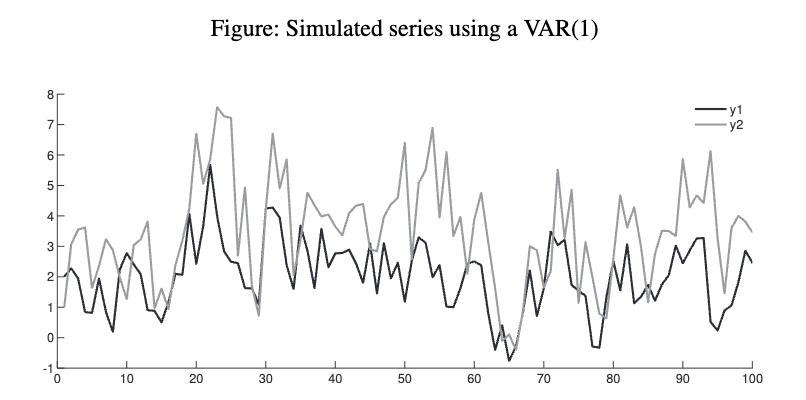
\includegraphics[width=0.8\textwidth]{2026-02-25-10-27-54.png}
\end{figure}
As the process is stable by definition, more on this later, both series $y_{1, t}\text{ and }y_{2, t} $ fluctuate around a constant mean, and their variability does not change as they wander along 

\subsection{The companion form}
\begin{itemize}
    \item VAR($p $) models, with $p > 1 $, can be written as VAR(1) models by employing the so-called companion form 
    \item Using the companion form simplifies notation and some derviations 
    \item A VAR($p $):
    \begin{gather*}
        y_t = \mu + A_1y_{t - 1} + A_2y_{t - 2} + \dots + A_pt_{p - 1} + e_t
    \end{gather*}
    can be written as a VAR(1): 
    \begin{gather*}
        \vec{Z_t} = \Gamma_0 + \Gamma_1Z_{t - 1} + v_t
    \end{gather*}
    \item How? Stack the vector $(y_t, y_{t - 1}, \dots, y_{t - p}) $ in the $Kp\times 1 $ vector $\vec{Z}_t $ as follows:
    \begin{gather*}
        \vec{Z}_t = 
        \begin{bmatrix}
            y_t \\ y_{t - 1} \\\vdots \\ y_{t - p + 1}
        \end{bmatrix}
        = 
        \begin{bmatrix}
            y_{1, t}\\
            y_{2, t}\\
            \vdots \\ 
            y_{K, t}\\
            \vdots \\ 
            y_{1, t - p + 1}\\
            y_{2, t - p + 1}\\
            \vdots \\
            y_{K, t - p + 1}\\
        \end{bmatrix}
    \end{gather*}
\end{itemize}
\newpage 
\begin{itemize}
    \item Writing out the matrices: 
    \begin{gather*}
        \begin{bmatrix}
            y_t \\ y_{t - 1} \\\vdots \\ y_{t - p + 1}
        \end{bmatrix}
        = 
        \begin{bmatrix}
            \mu \\ 0 \\\vdots \\ 0
        \end{bmatrix}
        +
        \begin{bmatrix}
            A_1 & A_2 & \dots & A_{p - 1} & A_p\\
            I & 0 & \dots & 0 & 0\\
            \vdots & \vdots & \ddots & 0 & 0\\
            0 & 0 & \dots & I & 0
        \end{bmatrix}
        \begin{bmatrix}
            y_{t - 1}\\ y_{t - 2} \\\vdots \\ y_{t - p}
        \end{bmatrix}
        +
        \begin{bmatrix}
            e_t \\ 0 \\ \vdots \\ 0
        \end{bmatrix}
    \end{gather*}
    \item Accordingly, the dimensions of the vectors $Z_t, \Gamma_0 \text{ and } v_t \text{ are } Kp\times 1 $. $A_j \text{ for } j = 1,\dots, p \text{ is } K\times K, \text{ and } \Gamma_1 \text{ is } Kp\times Kp $
    \item $\Gamma_1 $ is the companion form matrix 
    \item We also covered this when talking about AR processes. Same thing here, but multivariate.
\end{itemize}
\subsection{Stability of VARs}
\begin{itemize}
    \item As in the multivariate case AR($p $), we most often want the VAR($p $) to be covariance stationary
    \item For this to happen, the effects of shocks $e_t $ must die out 
    \item How to check for stationarity?
\end{itemize}
\textbf{Stationarity:}

Stationarity $\iff $ eigenvalues of the companion form matrix are all less than one in absolute value 
\begin{itemize}
    \item The eigenvalues are those numbers $\lambda $ for which: 
    \begin{gather*}
        |\Gamma_1 - \lambda I| = 0
    \end{gather*}
    \item Example, using numeric values from above: 
    \begin{gather*}
        \det\left(
            \begin{bmatrix}
                0.5 & 0 \\
                1 & 0.2
            \end{bmatrix}
            -\lambda
            \begin{bmatrix}
                1 & 0 \\
                0 & 1
            \end{bmatrix}
        \right)
        = \det \left(
            \begin{bmatrix}
                0.5 - \lambda & 0 \\ 
                1 & 0.2 - \lambda
            \end{bmatrix}
        \right)\\
        = (0.5 - \lambda)(0.2 - \lambda) = 0\\
        \to \lambda_1 = 0.5, \quad\lambda_2 = 0.2
    \end{gather*}
\end{itemize}
\newpage 
\subsection{Moving average representation}
\begin{itemize}
    \item Assuming that the VAR($p $) model is stable, we can derive its infinite moving average representation
    \item Two ways: recursive substitution or using lag operators 
    \item Again, this mirrors the result for the univariate AR case 
\end{itemize}
\subsubsection{Moving average by recursive substitution}
\begin{itemize}
    \item Assume VAR(1): 
    \begin{gather*}
        y_t = \mu + A_1Y_{t - 1} + e_t
    \end{gather*}
    \item Recursive substitution gives: 
    \begin{gather*}
        y_t = \left(I + A_1 + A_1^2 + \dots A_1^j\right)\mu + A_1^{j + 1}y_{t - (j + 1)} + e_t + A_1e_{t - 1} + A_1^2e_{t - 2} + \dots + A_1^je_{t - j}
    \end{gather*}
    where $A_1^0 = I $
    \item Stability implies $\left(I + A_1 + A_1^2 + \dots A_1^j\right)\mu\to(I - A_1)^{-1}\mu $ as $j\to\infty, \text{ and}, A_1^{j + 1}y_{t - (j + 1)}\to 0\text{ as }j\to\infty $
    \item Hence, 
    \begin{gather*}
        y_t = v + \sum_{j = 0}^{\infty}A^j_1e_{t - j}
    \end{gather*}
    where $v = (I - A_1)^{-1}\mu $
\end{itemize}
\subsubsection{Moving average representation using lag operators}
\begin{itemize}
    \item VAR(1) using lag operators: 
    \begin{gather*}
        (I - A_1L)y_t = \mu + e_t
    \end{gather*}
    which is often written: 
    \begin{gather*}
        A(L)y_t = \mu + e
    \end{gather*}
    Thus, $(I - A_1L) = A(L)$ (VAR($p $)):
    \begin{gather*}
        A(L) = (I - A_1L - A_2L^2 - \dots - A_pL^p)
    \end{gather*}
    \item Multiplying with $A(L)^{-1} $, we get the vector moving average representation: 
    \begin{gather*}
        y_t = A(L)^{-1}\mu + A(L)^{-1}e_t = B(L)\mu + B(L)e\\
        = v \sum_{j = 0}^{\infty}B_Je_{t - j}
    \end{gather*}
    \item using the geometric rule: 
    \begin{gather*}
        A(L)^{-1} = (I - A_1L)^{-1} = \sum_{j = 0}^{\infty}A_0^jL^j \equiv B(L) = \sum_{j = 0}^{\infty}B_jL^j
    \end{gather*}
    with $B_0 = I\text{ and }v = \left(\sum_{j = 0}^{\infty}B_j\right)\mu $
\end{itemize}
\newpage 
\subsection{Finding the MA coefficients}
\begin{itemize}
    \item The VAR(1) written in terms of the moving average coefficients:
    \begin{gather*}
        y_t = v + \sum_{j = 0}^{\infty}B_je_{t - j}
    \end{gather*}
    where $B_j = A_1^j, \text{ and }B_0 = I $
    \item How can we determine the $B_j $s, i.e., the moving average coefficients?
    \item Use the relationship $I = B(L)A(L) $, which holds due to the result above: 
    \begin{gather*}
        A(L)^{-1} = B(L)\Rightarrow I = B(L)A(L)
    \end{gather*}
    because $A(L)^{-1}A(L) = I $. Thus, 
    \begin{gather*}
        I = \left(B_0 + B_1L + B_2L^2 + \dots\right)\left(I - A_1L - A_2L^2 - \dots - A_pL^p\right)\\
        = \left(B_0 + B_1L + B_2L^2 + \dots\right) - \left(B_0A_1L + B_1A_1L^2 + B_2A_1L^3 + \dots \right) - \left(B_0A_2L^2 + B_1A_2L^3 + \dots\right) - \dots\\
        = B_0 + (B_1 - B_0A_1)L + (B_2 - B_1A_1 - B_0A_2)L^2 + \dots + \left(B_i - \sum_{j = 1}^{\infty}B_{i - j}A_j\right)L^i + \dots 
    \end{gather*}
    Solving for the relevant lags (noting that $A_j = 0 \text{ for } j > p $), we get: 
    \begin{align*}
        L^0 : B_0 &= I\\
        L^1 : B_1 &= B_0A_1\\
        L^2 : B_2 &= B_1A_1 + B_0A_2\\
        \Downarrow\\
        L^i : B_i &= \sum_{j = 1}^{i}B_{i - j}A_j\quad\text{for }i = 1,2, \dots
    \end{align*}
\end{itemize}
\subsection{The first and second order moments of VAR}
From above: MA representation gives 
\begin{gather*}
    y_t = v + \sum_{j = 0}^{\infty}B_je_{t - j}
\end{gather*}
with $v = \left(\sum_{j = 1}^{\infty}B_j\right)\mu = (I - A_1)^{-1}\mu $

\subsubsection{EV of the VAR}
Due to the Gaussian white noise asumption on the error terms, the EV of the process is simply: 
\begin{gather*}
    \mathbb{E}[y_t] = v = (I - A_1)^{-1}\mu 
\end{gather*}
This mean is sometimes described as the steady-state of the system 
\newpage 
\subsubsection{Covariance and autocovariance of VAR}
Define the covariance and autocovariance of the process by $Y $, which equals: 
\begin{gather*}
    Y(s) = \mathbb{E}[(y_t - v)(y_{t - s} - v)']\\
    = \mathbb{E}\left[\left(\sum_{j = 0}^{s - 1}B_je_{j - t} + \sum_{j = 0}^{\infty}B_{s + j}e_{t - s - j}\right)\left(\sum_{j = 0}^{\infty}B_je_{t - s - j}\right)'\right]\\
    = \sum_{j = 0}^{\infty}B_{s + j}\Sigma_eB_j'
\end{gather*}
\subsection{The autocorrelation function}
Normalization of $Y(s) $ gives the autocorrelation function: 
\begin{gather*}
    R(s) = D^{-1}Y(s)D^{-1}
\end{gather*}
where $D $ is the square root of the diagonal elements of $Y(0) $
\section{Estimating VARs}
\begin{itemize}
    \item Can be done equation by equation using OLS: consistent and efficient when the errors are normally distributed 
    \item More formally, define: $Y = [y_1, \dots, y_T]\, A = [A_1: \dots: A_p],\, U = [e_1,\dots, e_T]\text{ and } Z = [Z_0, \dots, Z_{T - 1}] $ where: 
    \begin{gather*}
        Z_{t - 1}=
        \begin{bmatrix}
            y_{t - 1}\\
            y_{t - 2}\\
            \vdots\\
            y_{t - p}
        \end{bmatrix}
    \end{gather*}
    \item The model can be writen as 
    \begin{gather*}
        Y = AZ + U
    \end{gather*}
    and the OLS estimator of $A $ is defined as: 
    \begin{gather*}
        \hat{A} = [\hat{A}_1: \dots: \hat{A}_p] = YZ'(ZZ')^{-1}
    \end{gather*}
    \item Under standard assumptions, the OLS estimator $\hat{A} $ is consistent and asymptitically normally distributed: 
    \begin{gather*}
        \sqrt{T}\,\text{vec}\left(\hat{A} - A\right)\xrightarrow{d}N\left(0, \Gamma^{-1}\otimes\Sigma_e\right)
    \end{gather*}
    where $\xrightarrow{d} $ implies convergence in distribution and $ZZ' / T \xrightarrow{p}\Gamma $
    \item Accordingly, standard inference applies to the estimated VAR parameters
    \item When no parameter restrictions are employed on the VAR system, and for a normally distributed Gaussian stationary process $y_t $, the OLS estimator is identical to the MLE conditional on the initial values. 
\end{itemize}
\newpage 
\subsection{Lag selection and testing}
\begin{itemize}
    \item VARs can be esitmated equation by equation using OLS 
    \item VAR models are heavily parameterized: 
    \begin{itemize}
        \item Significant tests on individual coefficients not necessarily very informative (depends on usage)
        \item More important to check properties of residuals: does the lag structure correctly capture the dynamics?
    \end{itemize}
    \item How many lags?
    \begin{itemize}
        \item Use information criteria (BIC, AIC, etc)
        \item Check properties of residuals (i.e., whiteness and autocorrelation)
    \end{itemize}
\end{itemize}
\section{Forecasting with VARs}
\begin{itemize}
    \item Again, this mirrors the results for the univariate AR case 
    \item Iterating the VAR forward: 
    \begin{gather*}
        y_{t + h} = \left(I + A_1 + \dots + A_1^{h - 1}\right)\mu + A_1^hy_t + \sum_{i = 0}^{h - 1}A_1^ie_{t + h - i}
    \end{gather*}
    \item Thus, the forcast $h = 01, \dots, H $ is a functino of $I(t) $ (the information set at time $t $ only)
    \item Note: the above equation is valid only for a VAR(1) process. Use companion form for more degrees processes and the formula remains unchanged 
\end{itemize}
\subsection{Point forecasts}
\begin{itemize}
    \item By employing the conditional expectation to the equation above, we get the VAR point forecast: 
    \begin{gather*}
        \mathbb{E}[y_{t + h}|y_t] = \left(I + A_1 + \dots + A_1^{h - 1}\right)\mu + A1^hy_t
    \end{gather*}
    \item $\mathbb{E}[y_{t + h}|y_t] $ is often called the predictor and is simply denoted $y(h)$
\end{itemize}
\subsubsection{Convergence of point forecast}
Under the maintained assumption about stationarity, the point forecasts converge to the unconditional mean of the process when $h $ goes to infinity: 
\begin{gather*}
    \mathbb{E}[y_{t + h}|y_t] = \frac{\mu}{I - A_1}\text{ when }h\to\infty
\end{gather*}
Again, tehse equations are just the multivariate extensions of the univariate case 
\newpage 
\subsection{Forecast errors and the MSE}
\begin{itemize}
    \item We are also interested in the forecast error and its variance, i.e., the MSE 
    \item The VAR forecast error at horizon $ h $ is:
    \begin{gather*}
        y_{t + h} - y(h) = \sum_{i = 0}^{h - 1}A_1^ie_{t + h - i}
    \end{gather*}
    Using the expectations operator: 
    \begin{gather*}
        \mathbb{E}[y_{t + h} - y(h)] ? \mathbb{E}[y_{t + h}] - \mathbb{E}[y(h)] = 0
    \end{gather*}
    Thus, the predictor $y(h) $ is unbiased 
\end{itemize}
\subsubsection{MSE}
\begin{itemize}
    \item The MSE is simply the forecast error variance, denoted $\Sigma_y(h) $:
    \begin{gather*}
        \Sigma_y(h) = \mathbb{E}\left[\big(y_{t + h} - y(h)^2\big)\right] = \mathbb{E}\left[\left(\sum_{i = 0}^{h - 1}A_1^ie_{t + h - i}\right)\left(\sum_{i = 0}^{h - 1}A_1^ie_{t + h - i}\right)'\right]
    \end{gather*}
    $\mathbb{E}[e_{t + h - i}] = \Sigma_e$ for all $h $, thus: 
    \begin{gather*}
        \Sigma_y(h) = \sum_{i = 0}^{h - 1}\left(A_1^i\Sigma_e A_1^{i\prime}\right)
    \end{gather*}
\end{itemize}
\subsection{The MSE and MA representation}
\begin{itemize}
    \item Expanding 
    \begin{gather*}
        y_t = A(L)^{-1}\mu + A(L)^{-1}e_t = B(L)\mu + B(L)e\\
        = v \sum_{j = 0}^{\infty}B_Je_{t - j}
    \end{gather*}
    and move it $h $ periods forwards, we get: 
    \begin{gather*}
        y_{t + h} = v + e_{t + h} + B_1e_{t + h - 1} + B_2e_{t + h - 2} + \dots + B_{h - 1}e_{t + 1} + B_he_t + B_{h + 1}e_{t - 1} + \dots
    \end{gather*}
    Computing the forecast gives: 
    \begin{gather*}
        y_{t +h} - \mathbb{E}\big[(y_{t + h} - \mathbb{E}[y_{t + h}|y_t])(y_{t + h} - \mathbb{E}[y_{t + h}|y_t])'\big] = \sum_{j = 0}^{h - 1}\left(B_j\Sigma_e B_j^{\prime}\right)
    \end{gather*}
\end{itemize}
\subsubsection{Convergence of MSE}
When $h\to\infty $, the equation above is equal to $Y(0) $, the unconditional variance of the VAR process. In mathematical terms: 
\begin{gather*}
    \Sigma_y(h) = Y(0)\text{ when }h\to\infty 
\end{gather*}
\newpage 
\subsection{Forecast intervals}
\begin{itemize}
    \item Assuming that the errors of the VAR model are Gaussian, i.e., $e_t\sim N(0, \Sigma_e) $, and independent across time, implies that the forecast errors are also normally distributed, such that: 
    \begin{gather*}
        \frac{y_{k, t + h} - y(k, h)}{\sigma_{y, k}(h)}\sim N(0, 1)
    \end{gather*}
    where $y_{k, t + h} \text{ and } y(k, h)$ are the $k $'th elements of the actual and predictor values, respectively, and $\sigma_{y, k}(h) $ is the square root of the variance for the $k $'th equation. That is, the square root of the $k $'th element on the diagonal of the $\Sigma_y(h) $ matrix. 
    \item Forecast intervals can be generated around the VAR point forecasts using 
    \begin{gather*}
        \big[y(k,h) - z_{\alpha/2}\sigma_{y, k}(h),\; y(h, k) + z_{\alpha / 2}\sigma_{y, k}(h)\big]
    \end{gather*}
\end{itemize}
\subsection{Forecasting with VARs: an example}
\begin{figure}[H]
    \centering
    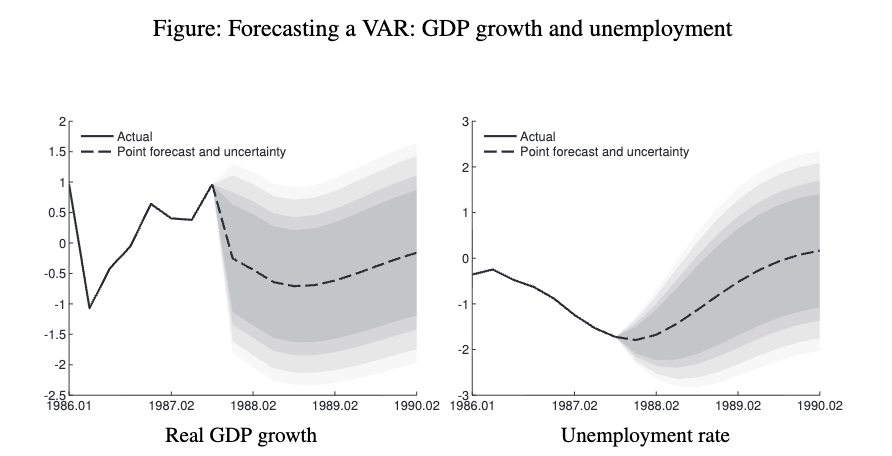
\includegraphics[width=0.8\textwidth]{2026-02-25-16-21-40.png}
\end{figure}
\textit{Note: The fan charts correspond to the 30, 50, 70 and 90 percent quantiles of the forecast distribution, with the darkest shade corresponding to the smalles quantile (30 percent). }
\newpage 
\section{Granger causality}
\begin{itemize}
    \item Cause cannot come after effect $\Rightarrow $ if $x $ causes $y, x $ should help predict $y $
    \item Granger causality $\Rightarrow $ predictability test!
    \item Consider the VAR system: 
    \begin{gather*}
        A_1 = 
        \begin{bmatrix}
            0.5 & 0\\
            1 & 0.2
        \end{bmatrix}
    \end{gather*}
    $y_{1, t} $ is not a function of past $y_{2, t} $, i.e., $y_{2, t} $ does not help predic $y_{1, t} $. However, $y_{2, t} $ is a function of past $y_{1, t} $, and therefore $y_{1, t} $ does help predict $y_{2, t} $. Accordingly, following the definition of Granger causality, $y_{1, t} $ does Granger cause $y_{2, t} $, but $y_{2, t} $ does not cause $y_{1, t} $
    \item Alternatively, if the coefficient matric had been: 
    \begin{gather*}
        A_1 = 
        \begin{bmatrix}
            0.5 & 0.2\\
            1 & 0.2
        \end{bmatrix}
    \end{gather*}
    both $y_{1, t} \text{ and } y_{2, t}  $ would have Granger caused each other. In this case we often say that the system for $y_t $ is a feedback system. 
    \item In practival situations the VAR representation has to be estimated 
    \item A test for Granger causality is implemented by employing a joint hypothesis test: 
    \begin{itemize}
        \item For each equation in the VAR we compare $K - 1 $ restricted versions of the VAR model against the unrestricted version 
        \item The test, for each restricted version, is a joint hypothesis test that all the lags of the $k $'th variable in the system are jointly significantly different from zero. As such, this is simply a standard $F $-test, where the null hypothesis is no Granger causality.
    \end{itemize}
\end{itemize}
\subsection{Example}
\begin{itemize}
    \item Assume a VAR(2) model, with three variables, the first equation of the system reads: 
    \begin{gather*}
        y_{1, t} = \mu_1 + \alpha_{11}y_{1, t - 1} + \alpha_{12}y_{2, t - 1} + \alpha_{13}y_{3, t - 1} + \alpha_{14}y_{1, t - 2} + \alpha_{15}y_{2, t - 2} + \alpha_{16}y_{3, t - 2} + e_{1, t}
    \end{gather*}
    \item The test for no Granger causality from $y_{2, t} \text{ to } y_{1, t} $ would be an F-test with $H_0: \alpha_{12} = \alpha_{15} = 0 $, and the test for no Granger causality from $y_{3, t}\text{ to }y_{1, t} $ would be an F-test with $H_0: \alpha_{13} = \alpha_{16} = 0 $. Conducting similar tests on the two other equations of the VAR representation would give a complete test for no Granger causality
    \item A rejection of any of the null hypotheses indicates Granger causality
\end{itemize}
\begin{figure}[H]
    \centering
    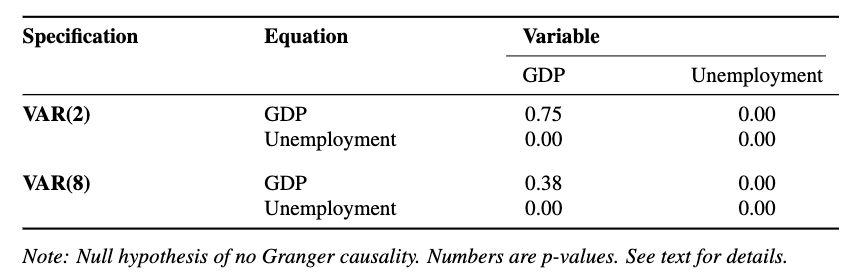
\includegraphics[width=0.8\textwidth]{2026-02-25-17-42-56.png}
\end{figure}
Reject $H_0 $ of no Granger causality for all but in one case: GDP is not Granger causing itself
\newpage 
\section{Summary}
\begin{enumerate}
    \item The vector autoregression (VAR) is a multivariate version of the univariate autoregressive model model (AR)
    \item A VAR($p $) can be written as a first order VAR(1) model by wriiting it in the companion form. 
    \item If all eigenvalues of the companion form matrix are less than 1 in absolute value, the VAR model is stable. A stable VAR model can be inverted and written as an infinite vector moving average model. 
    \item The VAR can be estimated by OLS equation-by-equation. Under standard assumptions, the OLS estimator will be similar to the MLE of the whole system 
    \item Testing for Granger causality involves testing whether or not lagged values of a given variable in the VAR system help predict one of the endogenous variables in the system. Such a test can simply be conducted using an F-test, where the null hypothesis is no Granger causality.
\end{enumerate}
\end{document}